\section{Why should we correct classifiers prediction}


we compared the result between 
\ref{eq:matchingfilter}
and
\ref{eq:matchingfiltercrossvalidation} 

Still, this last approach is not taking into account the quality of the classifier itself before taking into account its prediction. By this we ask the question of knowing how reliable the prediction of the classifier are? A common method to evaluate the uncertainty on the classifier prediction is to use a cross-validation procedure (see chapter~\ref{chapter:introduction:supervised}) to estimate the confusion matrix associated to the classifier. Such confusion matrix allow to infer the conditional probability of one label given the label prediction from the classifier $p(l^{cc} = l_k| l^c = l_q, \theta)$, for every combination of $k$ and $q$ in $1, \ldots, L$. Where $l^{cc}$ is the corrected, or ``temperated'', label predicted by the classifier given our estimates, our past experience, on the quality of its prediction using the cross validation procedure.

We consider the same setting as for the experiments described in chapter~\ref{chapter:bci:EEGsignals} and used our 2 dimensionnal dataset of different quality as presented in chapter~\ref{chapter:planning:artificialsignals}. We ran 500 simulations for each method.


% nSim =

%   Columns 1 through 3

%    104    98   123
%    115    96    90

%   Columns 4 through 5

%     86    89
%     83   117


\paragraph{Time to first task} Figure~\ref{fig:timefirst_simplevsmatching} compares the number of iterations needed to identify the first time with confidence between our general method (matching), or using the information that ``incorrect'' signals are more powerful than the ``correct'' (power), or both method combined (power matching). The use of the power information affects the performances for the low quality dataset. For datasets of low quality, while the time to first seems more advantageous for the method using the power information, most of the estimated task are erroneous (see Figure~\ref{tab:errorTaskRatio}) which makes the use of the power information critical for such low quality data. However those errors occurs for very low quality datasets, which are not the main target of our algorithm. For such data it would be better to change the representation of the signal or the classifier used. For the datasets of higher quality, the power information allow to slightly speed up the learning compared to our method (matching) which do not rely on known information. 

\begin{figure}[!ht]
\centering
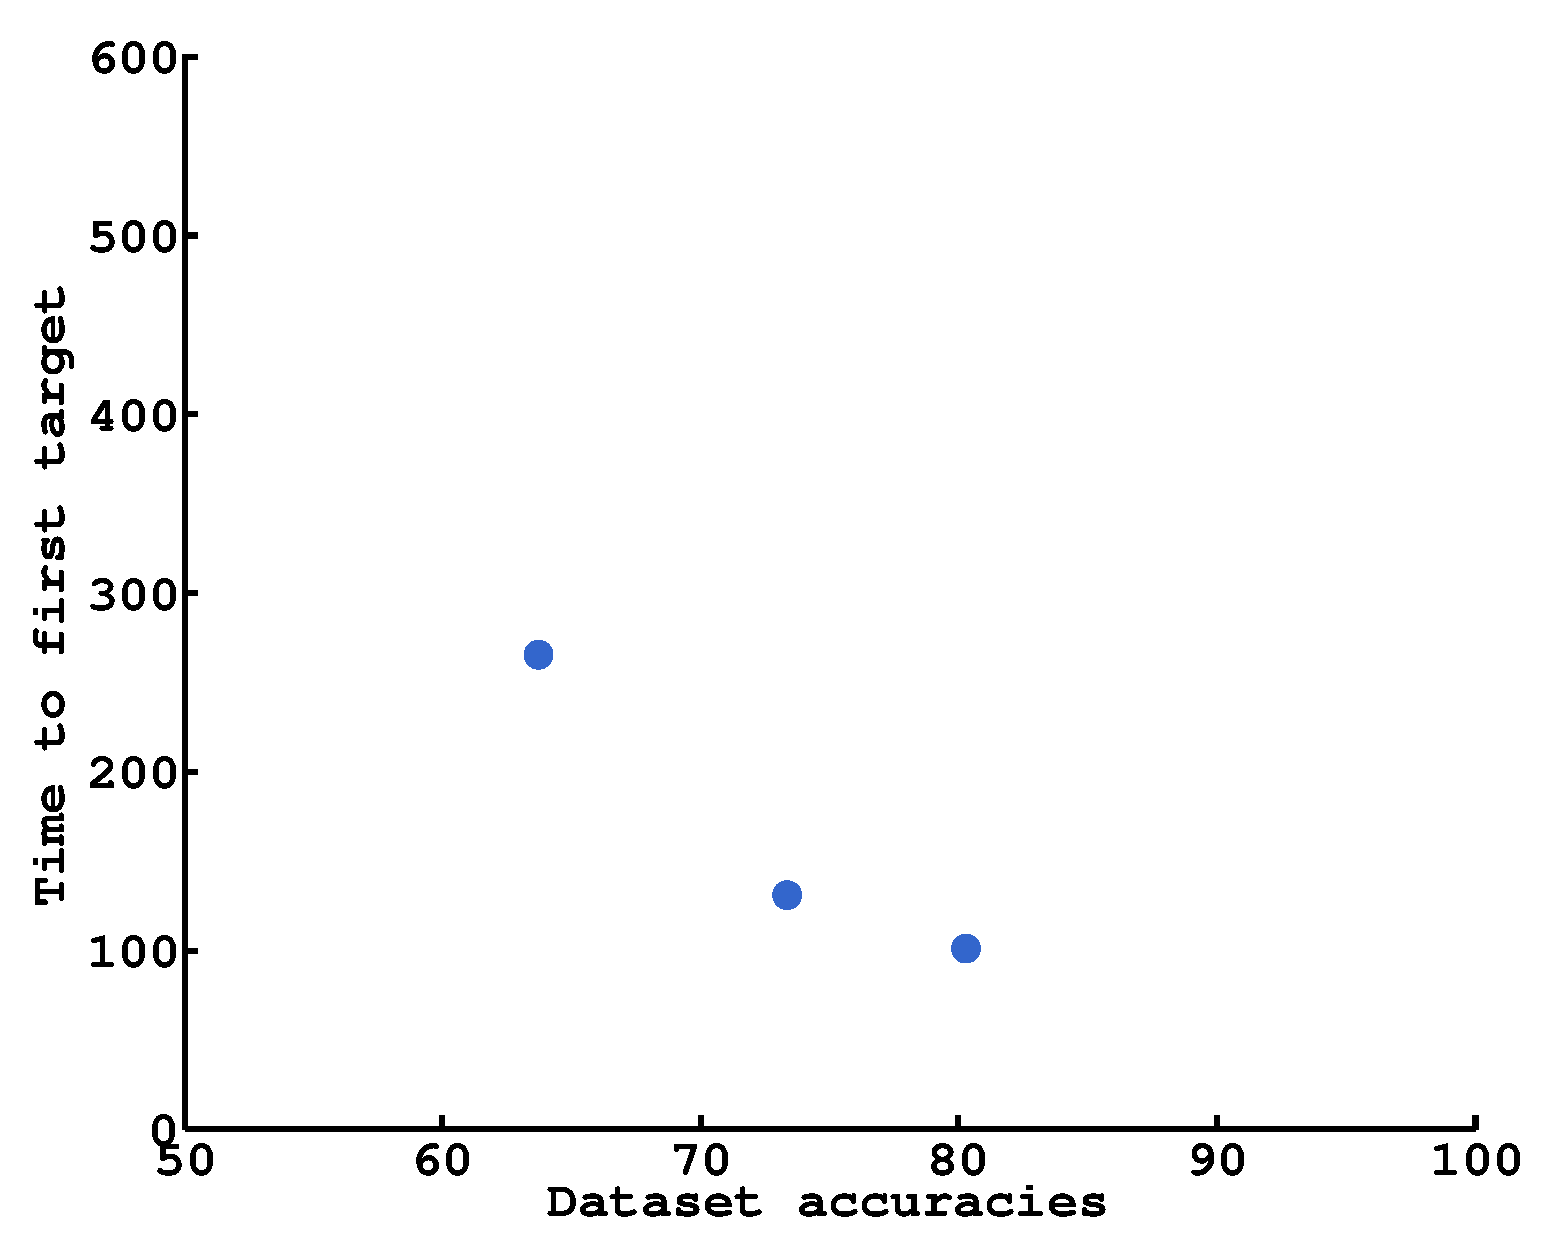
\includegraphics[width=\plotsize\columnwidth]{\imgpath/simplevsmatching/timefirst.eps}
\caption{Number of steps to complete first task with EEG data. Comparison between Equation~\ref{eq:matchingfilter} (simple matching) and Equation~\ref{eq:matchingfiltercrossvalidation} (matching), where the latter correct the prediction of the classifier given the estimation of its confusion matrix. 
% The use of the power information affects the performance for the low quality dataset. For datasets of low quality, while the time to first seems more advantageous for the method using the power information, most of the estimated task are erroneous (see Figure~\ref{tab:errorTaskRatio}) which makes the use of the power information critical for such low quality data. However those errors occurs for very low quality datasets, which are not the main target of our algorithm. For the datasets of higher quality, the power information allow to slightly speed up the learning compared to our method (matching) which do not rely on known information.
}
\label{fig:timefirst_simplevsmatching}
\end{figure} 

\begin{table}
\centering
\rowcolors{2}{gray!25}{white}
\begin{tabular}{c c c c}
    Dataset Accuracies & Simple Matching &  Matching \\ \hline
    50-60 & 0.21 & 0 \\ 
    60-70 & 0.16 & 0 \\
    70-80 & 0.03 & 0 \\
    80-90 & 0.02 & 0 \\
    90-100 & 0.01 & 0 \\
\end{tabular}
\caption{Percentage of time the first task estimated was erroneous using EEG data. Comparison between Equation~\ref{eq:matchingfilter} (simple matching) and Equation~\ref{eq:matchingfiltercrossvalidation} (matching), where the latter correct the prediction of the classifier given the estimation of its confusion matrix. Only our method that account temperate the prediciton fo the classifier do not make mistake when estimating the first task.}
\label{tab:errorTaskRatiosimplevsmatching}
\end{table}

\paragraph{Number of tasks achieved in 500 steps}

We compare the number of task correctly (Figure~\ref{fig:nCorrect_simplevsmatching}) and incorrectly (Figure~\ref{fig:nWrongEEG_simplevsmatching})reached in 500 steps between our general method (matching), or using the information that ``incorrect'' signals are more powerful than the ``correct'' (power), or both method combined (power matching). The power information makes more mistakes for low quality dataset which also impact the power matching method. However those errors occurs for very low quality datasets, which are not the main targets of our algorithm. For signals of above 60 percent classification rate, the power information improve the number of task we can reach. 

\begin{figure}[!ht]
\centering
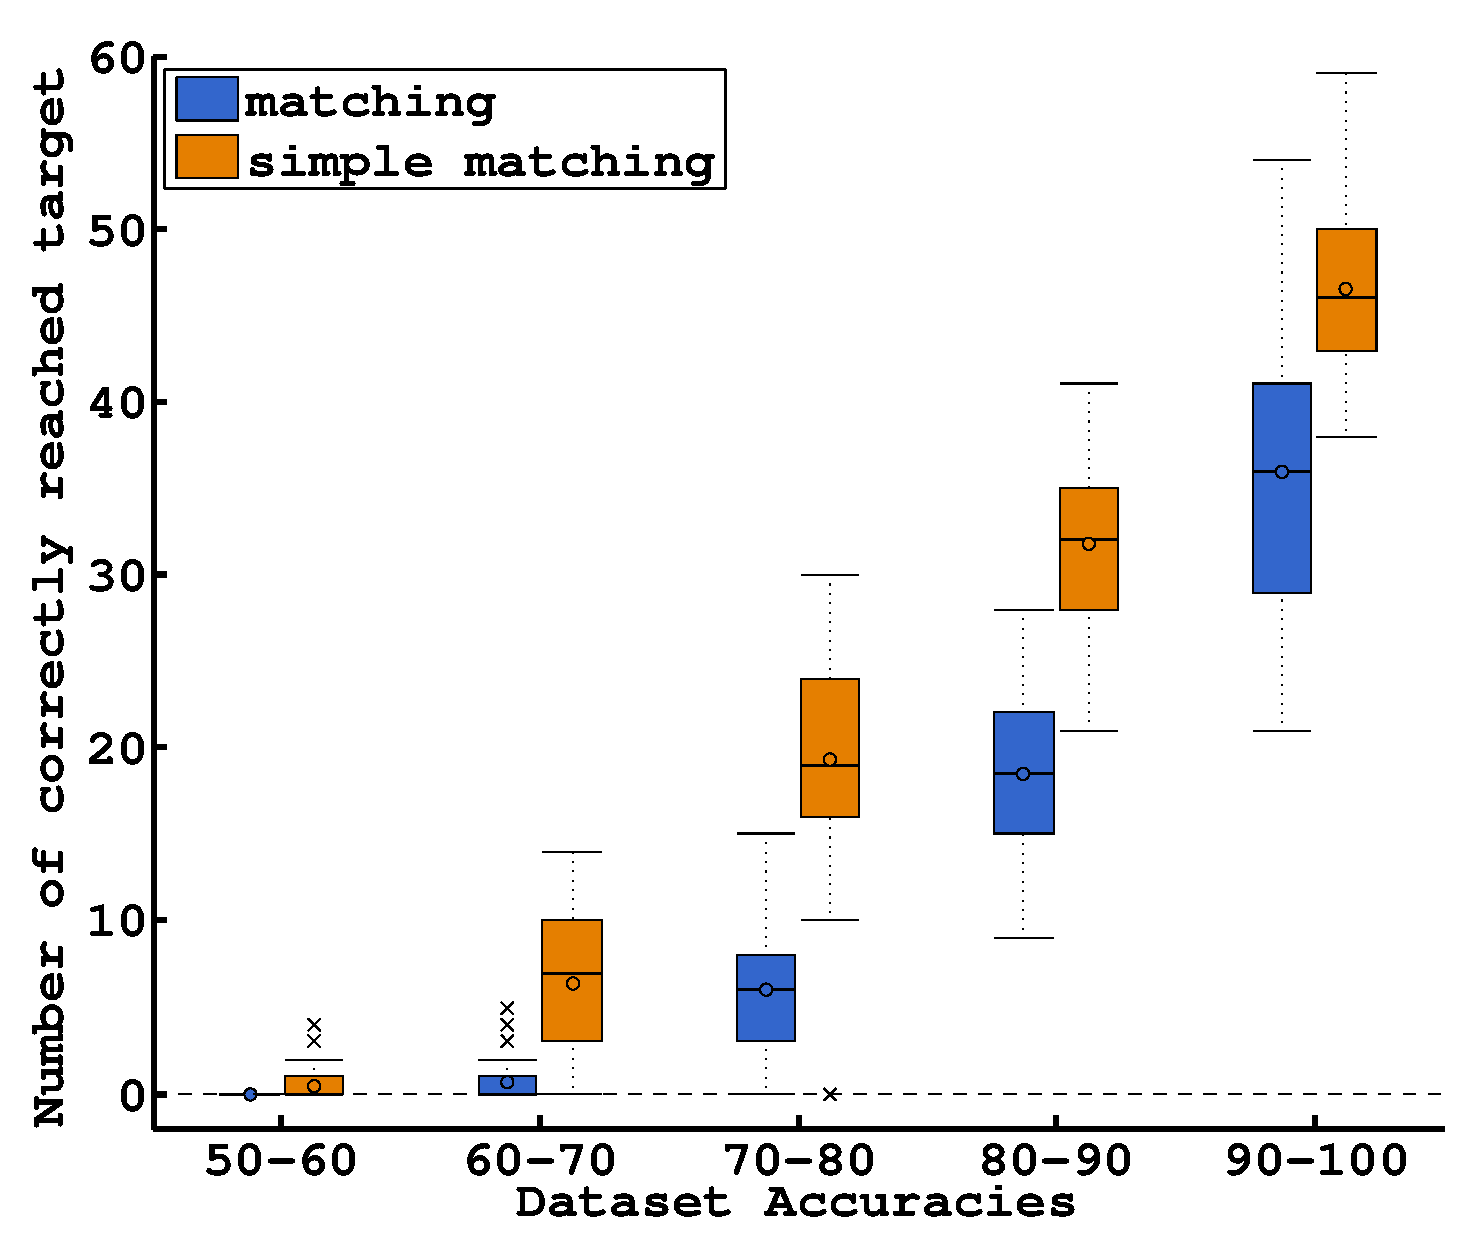
\includegraphics[width=\plotsize\columnwidth]{\imgpath/simplevsmatching/correct.eps}
\caption{Number of task correctly achieved in 500 steps with 2 dimensional artificial data. Comparison between Equation~\ref{eq:matchingfilter} (simple matching) and Equation~\ref{eq:matchingfiltercrossvalidation} (matching), where the latter correct the prediction of the classifier given the estimation of its confusion matrix. 
% The power information alone is sufficient to solve our problem but is less efficient than the other methods.
}
\label{fig:nCorrect_simplevsmatching}
\end{figure} 

\begin{figure}[!ht]
\centering
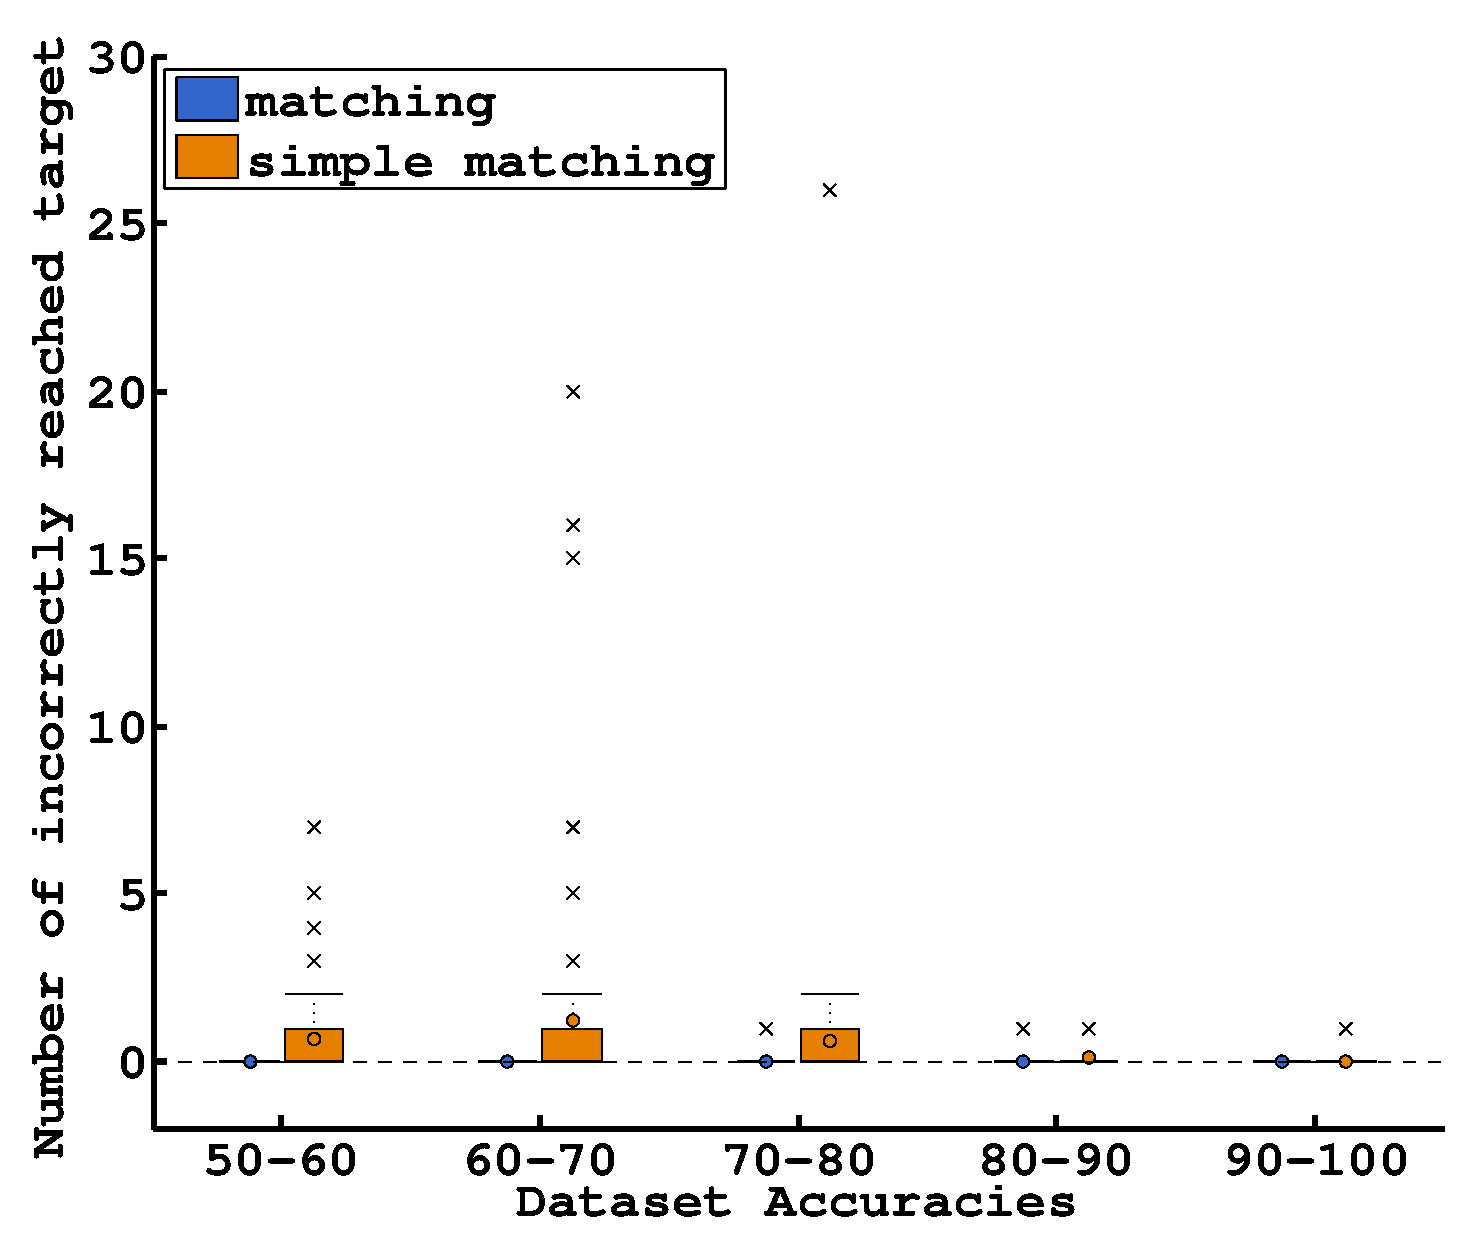
\includegraphics[width=\plotsize\columnwidth]{\imgpath/simplevsmatching/error.eps}
\caption{Number of task incorrectly achieved in 500 steps with 2 dimensional artificial data. Comparison between Equation~\ref{eq:matchingfilter} (simple matching) and Equation~\ref{eq:matchingfiltercrossvalidation} (matching), where the latter correct the prediction of the classifier given the estimation of its confusion matrix.
% The power information makes more mistakes for low quality dataset which also impact the power matching method. However those errors occurs for very low quality datasets, which are not the main targets of our algorithm.
}
\label{fig:nWrongEEG_simplevsmatching}
\end{figure} 


The power information alone is not enough to identify a high number of task, even if the number of steps to reach the first target are similar. The difference lies in the reallocation of labels we performed after a task is identified. As described in chapter~\ref{chapter:lfui:tasttotask}, once one task is identified with confidence we propagates its labels to all the other hypothesis. As a consequence, a majority of signal have identical labels, and the number of new signals with different labels needed to pull apart two hypothesis in terms of power ratio between classes increases. This is a problem resulting in measure relying only on global measure on the data. Our non-informed method (matching), measure the global quality of each classifiers but also consider the classification of each new signals individually, which speeds up the task reaching rate as the interaction goes on. See also the discussion of Figure~\ref{fig:sequence_evolution}.


Our results confirms that the use of the power information improves the performance of our algorithm. In addition, by disambiguating faster the task with symmetric properties, it also improves the visual impression our subjects get from the behavior of the agent with improved the quality of the signals received during our experimental test. At the time of writing those lines, this study was not over and this particular point requires a more detailed analysis to show and quantify this difference. It is particularly difficult to find a measure of perception of the agent behavior to quantify the difference between the use or not of the power information. We can only report here our experience from running the experiments, which is the reason of using the power information.


This is not possible with model method as the one presented in section~\ref{chapter:limitations:overlap}. Indeed to compute the prediction error of a model or a classifier, we need to compare its prediction with what is expected as a prediction. The labels outputted from our classifier can be compared with the label given in input. But for a model that output the probability of a particular signal, we can not compared the the true probabilistic value of each point and therefore we cannot quantify the prediction errors of such model.